\section{Contribution 2: Human pose estimation Kernel}

\subsection{Introduction}
In this brief section we describe the workings of the human detection system. It was developed by Etienne Pommel for a similar use case. The system is based on the mediapipe library \cite{mediapipe2020}, which is a state-of-the-art object detection algorithm that is capable of detecting humans in real-time. \cite{realsense_mediapipe}. The system is able to detect humans with high accuracy as they move around the environment. To the standard \gls{RGB} image, the system adds depth.

\begin{figure}[htbp]
    \centerline{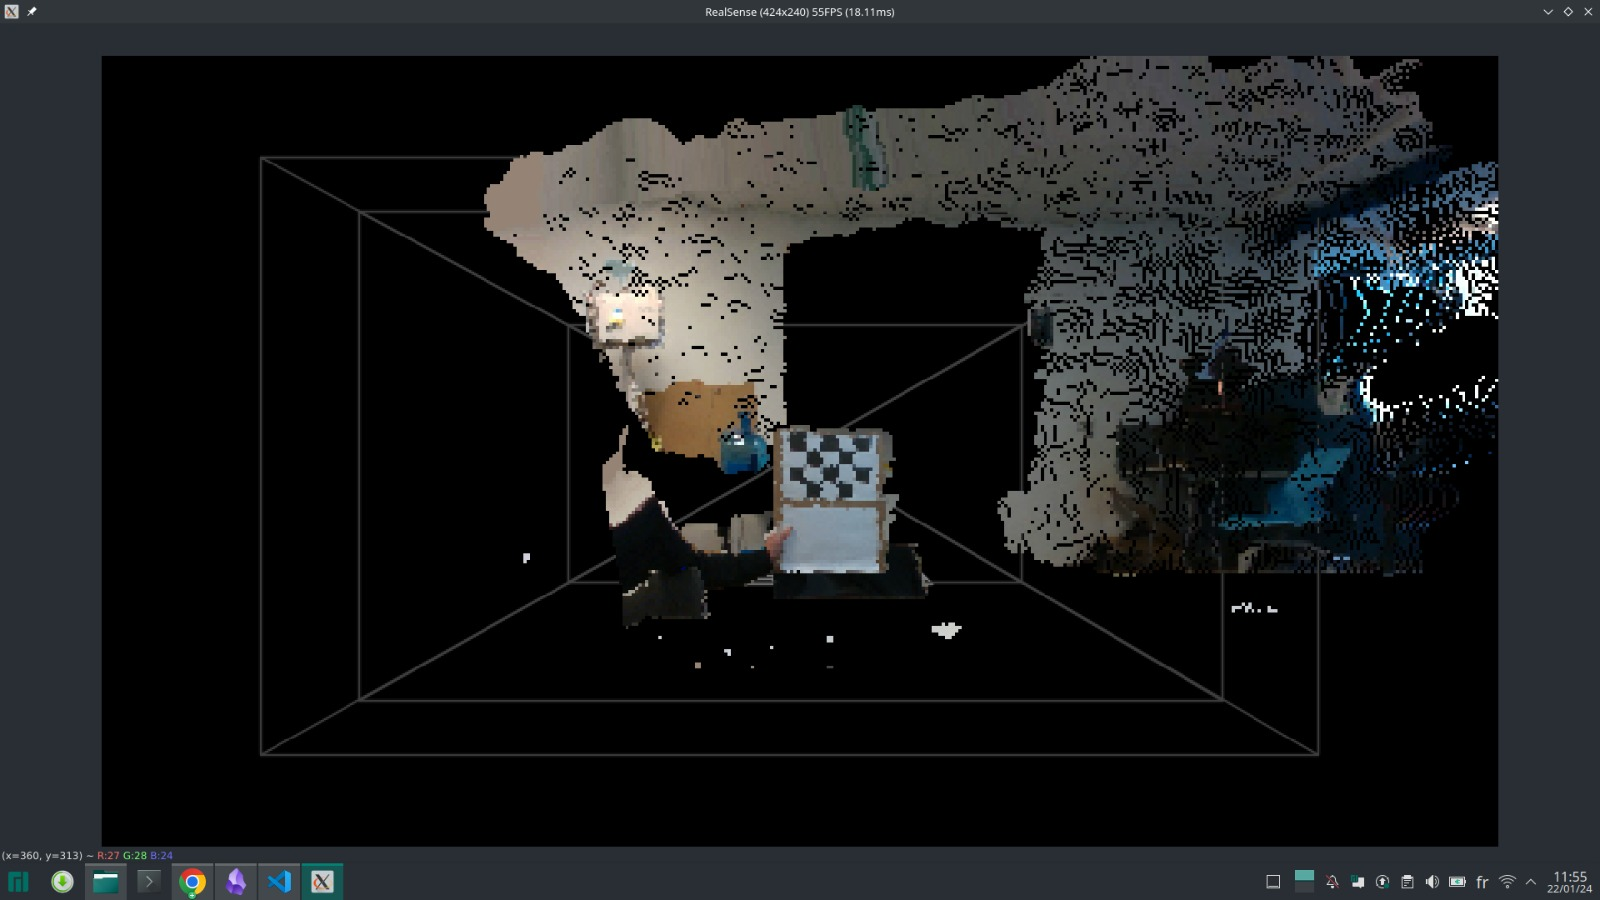
\includegraphics[width=1.0\textwidth]{images/rgbd.jpeg}}
    \caption{Intel Realsense D435, showing the workings of the depth camera and calibration capabilities, each pixel has been projected in the \gls{3D} space.}
    \label{fig}
    \end{figure} 
The difficulties of the system are to detect the objects in the image and to estimate the distance to the object. Finaly to project this distance in the \gls{3D} space.

Here we want to detect humans in the image this the use of mediapipe.

\subsubsection{Architecture}
The system was modified from the original algorithm as it would continuously calibrate using the chessboard.~\ref{appendix:additional_work}

\begin{figure}[htbp]
    \centerline{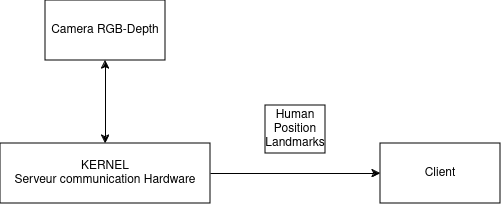
\includegraphics{images/objectschema.png}}
    \caption{Object Control Kernel, showing the main components of the system.}
    \label{fig}
    \end{figure} 
\begin{figure}[htbp]
    \centerline{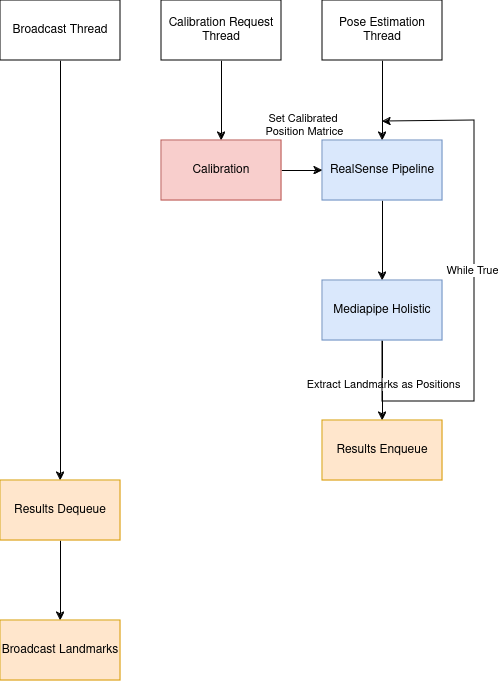
\includegraphics[width=0.5\textwidth]{images/ObjectRecognitionLogics.png}}
    \caption{Object Control Kernel, inside logics.}
    \label{fig}
    \end{figure} 

\subsection{Evaluation and Results}
Also a ThreeJS interface is provided to visualize the drones in \gls{3D} space. This interface allows users to see the humans' positions and orientations in real-time, providing a visual representation of the system's behavior. The ThreeJS interface communicates with the FastAPI application to receive updates on the humans' positions and orientations.

We have evaluated the components of the human detection kernel to ensure that they meet the requirements of the system. The results of the evaluation are presented in the following sections.

We expected the measures to be accurate to at least 5\% of the real distance but expect it to be less reliable the further the subject is to the camera. The system was not able to provide this much accuracy but 10\% at 5 meters. The system though was able to provide a good estimate of the distance to the object, constant at 2\% of the real distance at less then 7m.
\begin{figure}[htbp]
    \centerline{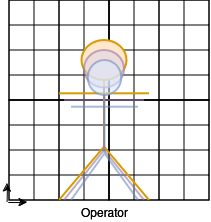
\includegraphics[width=0.3\textwidth]{images/humanreconitionflaw.png}}
    \caption{Object Control Kernel Issue, further the object is from the camera and the center of the image the smaller it will be estimated. The distance to the camera does not change only the size of the object in the image plane.}
    \label{fig}
    \end{figure} 
Indeed the results are less satisfying then expected but the system is still able to provide a good estimate of the distance to the object. The system is able to detect the object in the image and to estimate the distance to the object. The system is also able to project this distance in the \gls{3D} space, we will need to takee this into account in the next part of the project.

Similarly to the drones kernel, the system was made as stateless as possible. So after setup no command could break it. This system does not require a lot of resources and is able to send all the 30 landmarks per frame at the rate of 30 per second to the client so \[900 \text{ landmarks per second.}\]

\subsection{Conclusion} 
The human pose estimation kernel provides a valuable system for detecting and estimating the distance of humans in real-time, using the Mediapipe library in combination with depth sensors. While the results showed a degree of inaccuracy beyond 5 meters, the system successfully achieved consistent performance within 2\% accuracy for shorter distances (less than 7 meters). Despite some limitations—such as reduced reliability at greater distances and issues with object size estimation at image boundaries—the system still delivers an effective method for projecting human positions in \gls{3D} space. Future improvements should focus on enhancing the calibration mechanisms and addressing the accuracy drop at longer ranges, which will be vital for the next phase of the project.